\documentclass[12pt]{article}
\usepackage[letterpaper, portrait, margin=.5in]{geometry}
\usepackage[T1]{fontenc}
\usepackage{setspace}
\usepackage{fancyhdr}
 \usepackage{color}
\usepackage[dvipsnames]{xcolor}
\pagestyle{fancy}
\usepackage{multicol}
\usepackage{graphicx}
\usepackage[abspath]{currfile}[2012/05/06]
\thispagestyle{empty}
\graphicspath{{\currfileabsdir}}
\definecolor{glaucous}{rgb}{0.38, 0.51, 0.71}
\def\labelitemi{--}


\setlength{\columnseprule}{4pt}
\def\columnseprulecolor{\color{gray}}
\newcommand{\tab}[1]{\hspace{.1\textwidth}\rlap{#1}}

\begin{document}
\center
\begin{Huge}\textbf{Bryce John Sampson}\end{Huge}\\
\medskip
\fontsize{12}{1.2}
\selectfont

\noindent
sampson.bryce@yahoo.com | +1 530-859-5330 | Vallgatan 12A Room 805, Vaxjo Sweden 352 35
\noindent\rule{17cm}{0.4pt}\\
\smallskip
\textbf{GITHUB: \color{TealBlue}github.com/sampsonbryce}\\
\smallskip
\textbf{WEBSITE: \color{TealBlue}sampsonbryce.github.io}\\
\smallskip
\noindent\rule{17cm}{0.4pt}

\center
\textbf{\textsc{-Education-}}\\
\flushleft
\begin{footnotesize}
\textsc{California State University, Chico CA}
\hfill
\color{Cerulean}\textbf{Major GPA: }\color{black}3.95\\

\color{black}
\smallskip
\textsc{Linnaeus University, Vaxjo Sweden (2017-2018 Academic Year Abroad)}
\hfill
\color{Cerulean}\textbf{Cumulative GPA: }\color{black}3.77\\
\smallskip

\color{Cerulean}\textbf{Major: }\color{black}Computer Science
\hfill
\color{gray}Class Standing Senior: Expected Graduation Spring 2019\\
\smallskip

\end{footnotesize}

\smallskip

\noindent\rule{19cm}{0.4pt}
\bigskip
\begin{multicols}{2}
\begin{center}
\textbf{\textsc{-Skills-}}
\bigskip

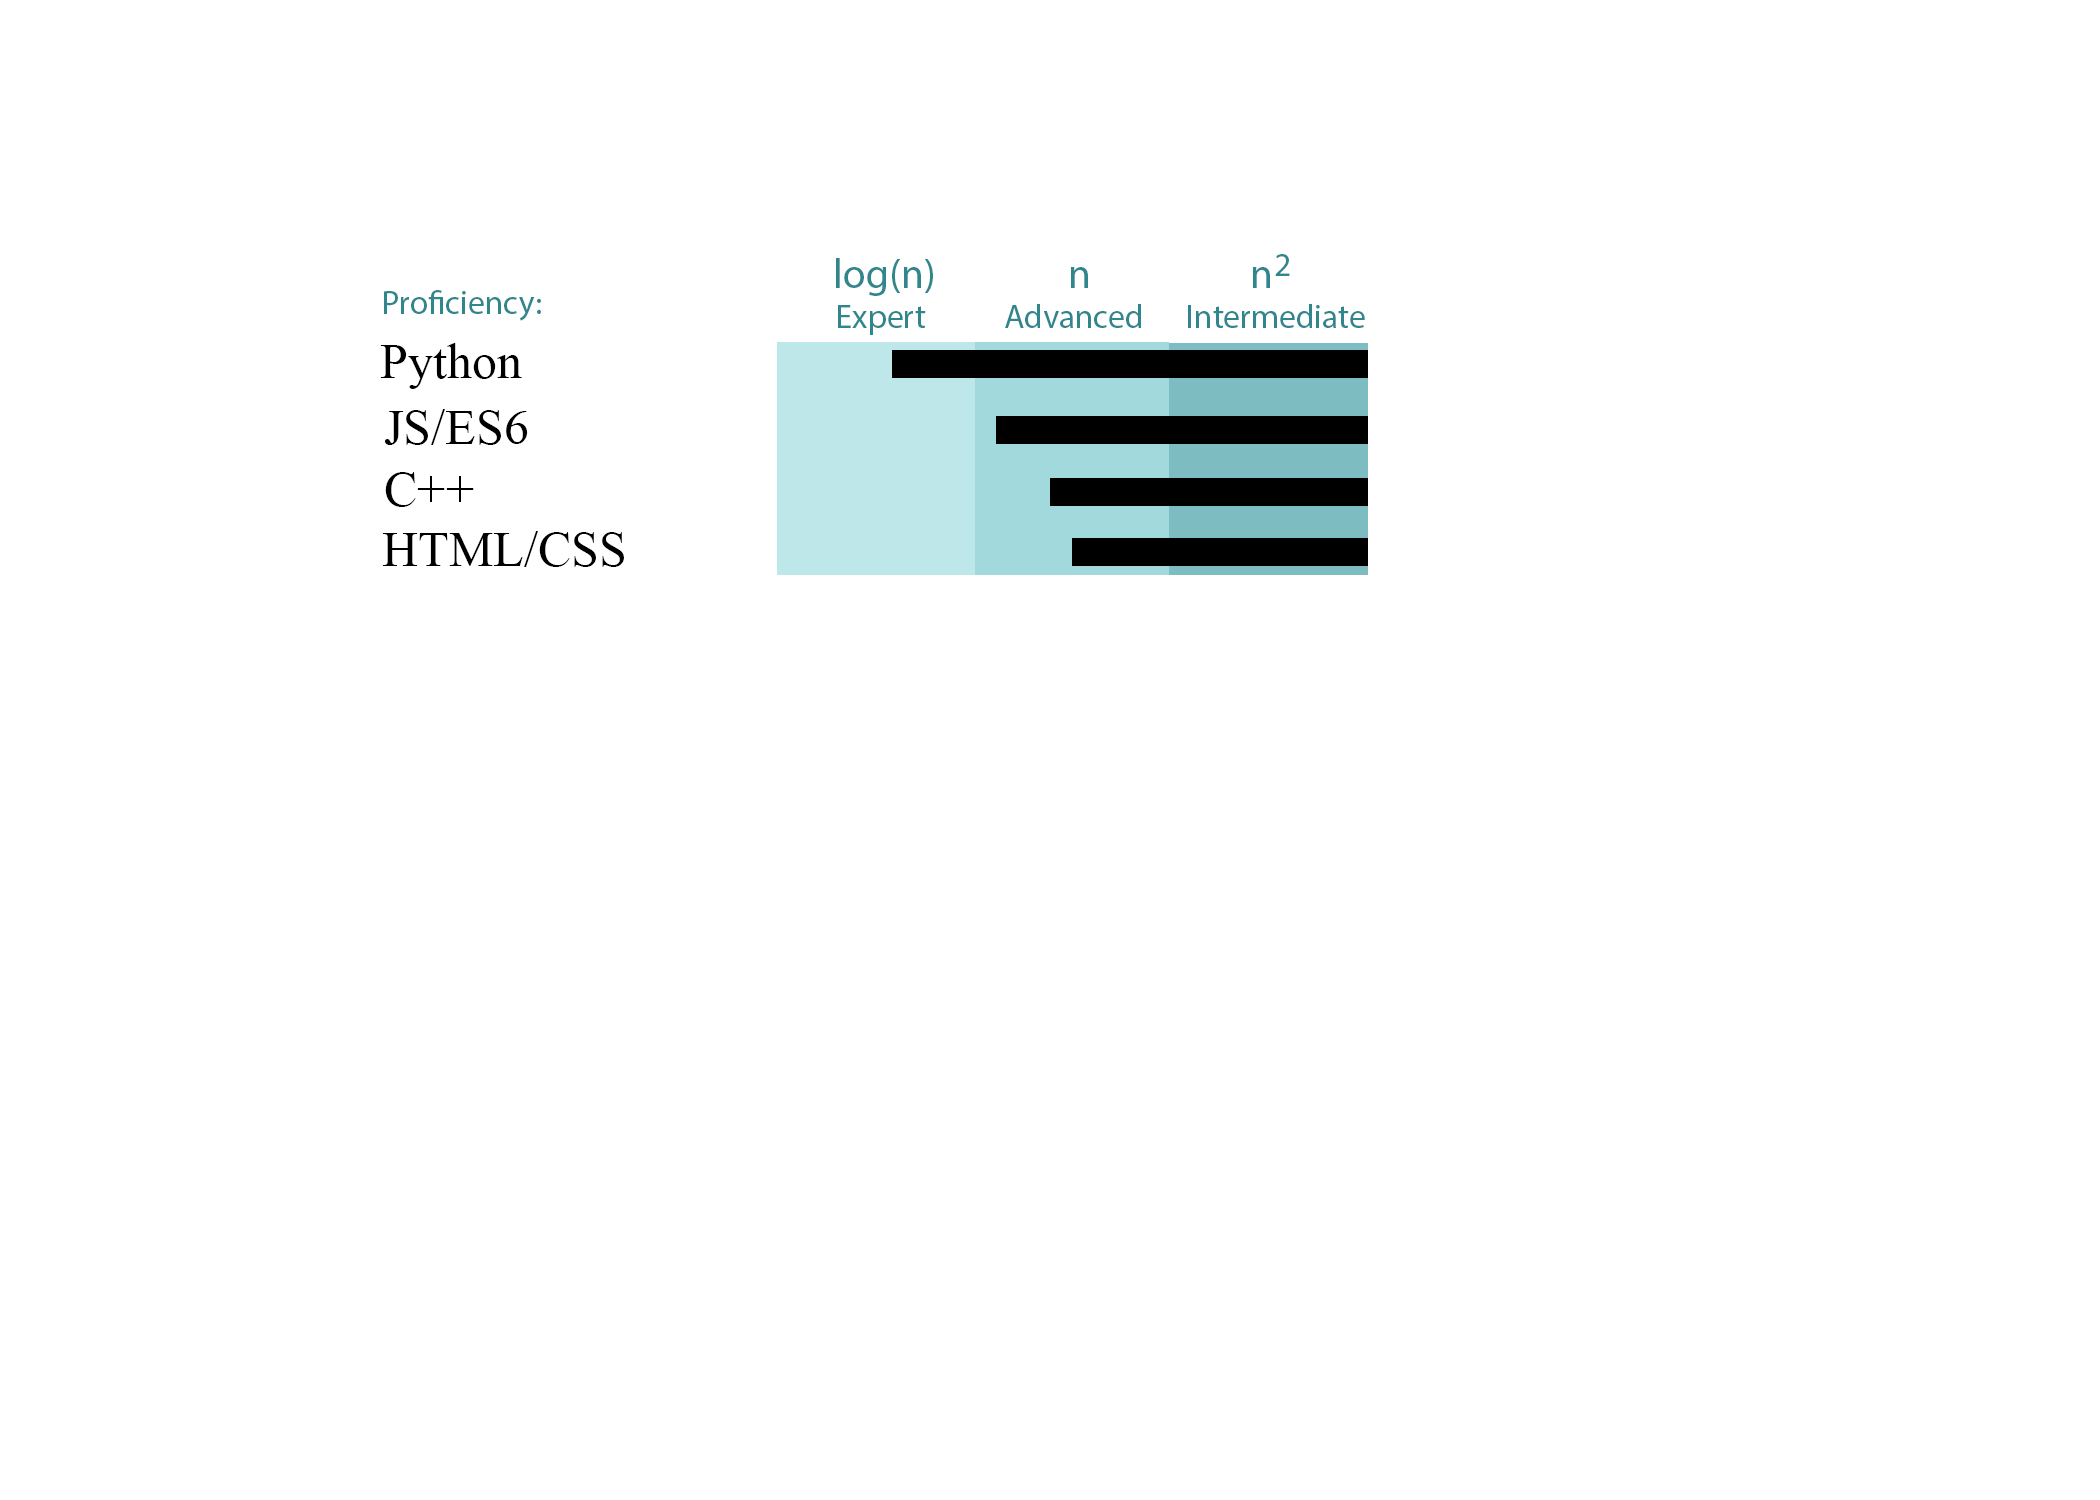
\includegraphics[trim={2.8cm 7cm 2cm 2cm},clip]{ResumePic.png}
\footnotesize
\color{gray}Git | Vim | Linux | Windows | MacOS | Android
\end{center}
\columnbreak
\center
\footnotesize
\color{black}\textsc{\textbf{ACM Club | CSU, Chico}}\\

\color{Cerulean}Algorithms Officer \hfill \color{gray}\textit{Spring 2017}\\
\begin{itemize}
\setlength{\itemsep}{0pt}
	\item Competed in Fall 2016 ACM Competition
	\item Research and present/teach algorithms at club meetings to be used during competition
\end{itemize}

\center
\color{black}\textsc{\textbf{Formula SAE Electric | CSU, Chico}}\\
\color{Cerulean}Member \hfill \color{gray}\textit{Spring 2017}

\begin{itemize}
\setlength{\itemsep}{0pt}
	\item Develop Formula SAE car to compete nationally
	\item Contribute to batteries and motor control team
\end{itemize}


\end{multicols}

\noindent\rule{19cm}{0.4pt}

\center
\color{black}
\color{black}
\begin{center}
\textbf{\textsc{-Internships-}}\\
\end{center}
\begin{footnotesize}
\flushleft
\color{Cerulean}\textbf{Workday Inc}\hfill \color{TealBlue} \textbf{Python | Bash} \\ 
\color{Black}\textit{Environments Engineer Intern} \hfill \textit{May 2017 - August 2017}
\color{black}
\begin{itemize}
    \setlength{\itemsep}{0pt}
	\item Developed internal environment management tools for Automation and Network Operations sub-team of the Environments department
	\item Provisioned and de-provisioned environments for Sales Environment team
\end{itemize}
\color{Cerulean}\textbf{SocialHighRise}\hfill \color{TealBlue} \textbf{HTML/CSS/JS | jQuery | ASP.NET MVC | C\# | Razor | WordPress } \\ \color{Black}\textit{Software Development Intern} \hfill \textit{August 2016 - May 2017}
\color{black}
\begin{itemize}
    \setlength{\itemsep}{0pt}
	\item Develop in-house account manangement tool for organizing and monitoring social media profiles
	\item Manage all company tech support and IT needs including company website development
\end{itemize}
\color{Cerulean}\textbf{Lawrence Livermore National Laboratory} \color{Black} \hfill
\color{TealBlue} \textbf{PySide Qt | Python | HTML/CSS/JS | jQuery | React/Redux}\\
\color{Black} \textit{Computation Intern} \hfill\textit{Jan 2016 - August 2016} 
\color{Black}
\begin{itemize}
    \setlength{\itemsep}{0pt}
	\item Employed in a Co-op position, developing a Graphical User Interface for a large scale climate data visualization and analysis tool developed at the lab.
	\item Developed GUI in both PySide Qt and from scratch in HTML/CSS/JS, jQuery, React/Redux, and Flask

	\item Organized and presented demos of project to our team and communicated development timeline
	\item Collaborated with scientists using alpha, beta and previous versions of GUI to improve user experience and implement new functionality
\end{itemize}

\end{footnotesize}

\noindent\rule{19cm}{0.4pt}

\begin{center}
\textbf{\textsc{-Projects-}}\\
\end{center}
\begin{footnotesize}

\flushleft

\color{Cerulean}\textbf{Hero Home (home.heroinc.io): \hfill\color{TealBlue} Vue.js | HTML/CSS | Node.js/Express | Nginx } 
\color{Black}
\begin{itemize}
	\item Chrome Extension and Home Page for Google search that displays advertisements to raise money for charity
\end{itemize}
\smallskip


\flushleft

\color{Cerulean}\textbf{Datasift Sentiment Visualization: \hfill \color{TealBlue} Node.js/Express | React | D3 | HTML/CSS/JS | jQuery} 
\color{Black}
\begin{itemize}
	\item Utilized Datasift Facebook Topic Data API trial to create visualization representing sentiment 
\end{itemize}
\smallskip

\end{footnotesize}

\center
Created with \LaTeX
\end{document}